 % arara: xelatex: {shell: true}
% arara: biber
% arara: xelatex: {shell: true}
% arara: xelatex: {shell: true}

% Podklad k cvičení v předmětu BI-DPR
% autor: Ondřej Guth (ondrej.guth@fit.cvut.cz)
% (c) FIT ČVUT, 2018


\documentclass[a4paper]{article}
\usepackage{polyglossia}
\setmainlanguage{czech}
\usepackage{xevlna,xltxtra}
\usepackage{csquotes}
%\usepackage[style=german]{csquotes} % pro starší verze, kde není čeština

\usepackage[hidelinks]{hyperref}
\usepackage{graphicx}
\usepackage{minted}
\usepackage{xfrac}
\usepackage{nicefrac}
\usepackage[style=iso-numeric]{biblatex}

\title{MI-PAA\\
\large Úkol 5 -- zpráva\\}

\author{Tomáš Přeučil}

\begin{document}

\maketitle

%\tableofcontents

\section{Zadání úlohy}
	Zadáním bylo řešení problému vážené splnitelnosti booleovské formule pokročilou iterativní metodou.\footnote{https://moodle.fit.cvut.cz/mod/assign/view.php?id=59201}

	K řešení měl být použit stejný algoritmus jako ve čtvrté úloze\footnote{https://github.com/tomaspre/MI-PAA/tree/master/tasks1to4} -- v tomto případě genetický.


\section{Použité prostředky}
	\subsection{Programovací jazyky a software}
		Úloha byla řešena v jazyce Python ve verzi 3.6 pod operačním systémem OS X 10.11.6. Program byl spouštěn z Bashe a tudíž pro spuštění nebylo využito žádné IDE.
		Pro měření času byla využita knihovna time a funkce \textit{time.process\_time()}. Jedná se o novinku od verze 3.3, která pracuje velmi podobně jako doporučovaná knihovna \textit{timeit}.
		
	\subsection{Konfigurace testovacího stroje}
		Testování bylo provedeno na MacBooku Pro 13", Early 2011, modelové číslo MC700LL/A. Stroj obsahuje CPU Intel Core i5 2415M (2,3~GHz) a 16~GB RAM. Jediný další rozdíl oproti výchozí konfiguraci je vyměněný disk (za SSD), což však v tomto případě nehraje roli.

\section{Rozbor algoritmu}
	Genetický algoritmus funguje tak, že postupně šlechtí co nejlepší jedince -- v tomto případě bitové vektory.
	
	Na začátku je nutné vytvořit počáteční populaci. To je možné udělat buď náhodně, nebo jedince \enquote{seedovat} do té oblasti stavového prostoru, kde by se mohlo nacházet řešení -- to je však zadáním silně nedoporučeno.
	
	Tato populace je dále šlechtěna. Jednak se dva jedinci mohou s určitou pravděpodobností křížit, ale také mohou mutovat. Po jednom cyklu šlechtění tedy máme generaci obsahující původní rodiče, mutanty a potomky. V tuto chvíli je nutné vybrat jedince pro další generaci.
	
	Popis konkrétní implementace a postup nastavení parametrů se nachází v dalších kapitolách.
	

\section{Popis postupu řešení}
	Jako kostra implementace posloužil algoritmus popsaný v minulé kapitole.
	
	\subsection{Implementace obecně}
		Idea byla vše maximálně zapouzdřit a využít tak objektových možností jazyka Python. První implementovanou třídou je třída \textit{problem}. Tato třída obsahuje řešenou formuli (dvojrozměné pole, či v případě pythonové terminologie spíše dvojrozměrný list), pole s vahami jednotlivých proměnných, proměnné udávající počet proměnných, počet klauzulí a pole objektů \textit{chromosome}.
		
		Toto pole má velikost danou velikostí populace. Každý objekt v sobě ukládá svou fitness, počet proměnných, odkaz na třídu \textit{problem} a bitový vektor pro uložení hodnot. Objekt \textit{chromosome} dále implementuje metody inicializace, mutace, křížení (druhým parametrem je jiný chromosom) a výpočtu fitness. Výpočet fitness je volán vždy na konci volání konstruktoru. Tím je dosaženo maximálního zapouzdření a v případě použití heuristiky pro jiný problém stačí vyměnit fitness funkci a inicializační část konstruktoru. Návrh objektu \textit{chromosome} funguje s libovolným objektem mající atribut \textit{present}.
		
		Výše zmíněná inicializační část je sama o sobě zajímavá. Pokud je konstruktor volán s příznakem \textit{init = 1}, je provedena inicializace bitového vektoru náhodným binárním řetězcem. To opět způsobuje další zapouzdření.
		
		Třída \textit{problem} implementuje jedinou metodu -- \textit{solve}. 
	
	\subsection{Implementační specifika}
		Tato podkapitola popisuje implementační specifika.
	
		\subsubsection{Fitness funkce}
			Pokud je formule splněna, je hodnotou fitness suma vah \enquote{jedničkových} formulí.
			
			Pokud formule splněná není, fitness je spočítána takto: $$(-1) * penalizace * pocet nesplnenych klauzuli$$
		
		\subsubsection{Běh algoritmu}
			Po vygenerování (náhodné) počáteční populace	je prováděn genetický algoritmus s určitými modifikacemi.
		
			Nejprve je pro každý chromosom rozhodnuto, zda bude křížen s nějakým jiným. Pokud má být chromosom křížen, je proveden turnajový výběr. Z $n$ náhodně vybraných možných druhých rodičů je vybrán ten s nejvyšší fitness. Důvod turnajového výběru pouze jednoho rodiče je experimentálně ověřená nižší pravděpodobnost uváznutí v lokálním optimu. Výsledkem křížení jsou dva noví potomci a velikost současné populace se tedy zvýší o 2.
		
			Dále je prováděna mutace. S určitou pravděpodobností může každý chromosom zmutovat a to tak, že je v něm změněn jeden náhodný bit. Tento \enquote{mutant} je pak přidán do populace a její velikost se tedy zvýší o 1.
		
			V následujícím kroku je pole chromozomů seřazeno dle fitness. Velikost populace je v tuto chvíli však vyšší než ta daná parametrem. Proto je náhodně vyřazeno tolik jedinců, aby došlo ke snížení velikosti populace na zadanou hodnotu. V rámci elitismu je nejlepší jedinec chráněn před vyřazením.
			
			Pokud se hodnota fitness za posledních $x$ kroků nezměnila a formule je splněna, je běh algoritmu ukončen.
			
			Pokud se hodnota fitness za posledních $z * x$\footnote{$z$ je konstanta, kterou je přenásoben parametr $x$ z minulého odstavce} kroků nezměnila a formule není splněna, je celá populace až na nejlepšího jedince přegenerována. To zajišťuje mnohem vyšší pravděpodobnost splnění formule.
		
	\subsection{Data}
		Implementovaný algoritmus bylo nejprve potřeba otestovat, zda dává správné výsledky. To se ukázalo, jako výrazně složitější, než by se mohlo zdát. Jako první byl implementován opravdu velmi jednoduchý generátor instancí o jednotkách proměnných a klauzulích.
		
		Na datech z tohoto generátoru se ukázalo, že formule o tomto rozsahu bývají buď nesplnitelné, nebo, dost často, mají ideální ohodnocení složené pouze z \enquote{jedničkových formulí}. Na těchto datech se tedy podařilo otestovat, že algoritmus dobře řeší obyčejný SAT, nikoli však např. relativní chybu sumy vah.
		
		Pro veškeré další testy byla použita data ze stránek The University of British Columbia.\footnote{https://www.cs.ubc.ca/~hoos/SATLIB/benchm.html} Kladné váhy byly dogenerovány náhodně.

	
\section{Výběr parametrů}
	Před použitím algoritmu je nutné nastavit všechny parametry. Tato kapitola popisuje popis nastavení. Na začátku je však nastavit všechny parametry na nějakou \enquote{bulharskou konstantu} (většinou byly použity hodnoty z minulé úlohy) a od této hodnoty se \enquote{odpíchnout}. Pro představu -- není možné zjišťovat ideální pravděpodobnost křížení pokud by algoritmus neměl zadanou nějakou hodnotu pro pravděpodobnost mutace.
	
	Úvodní nastavení (a seznam nastavitelných parametrů) je následující:
	\begin{itemize}
		\item velikost populace = 200,
		\item maximální počet populací = 350,
		\item penalizace za každou nesplněnou klauzuli = 10,
		\item pravděpodobnost mutace (\%) = 8,
		\item pravděpodobnost křížení (\%) = 70,
		\item maximální počet generací (když je formule splněna) beze změny nejlepší fitness = 20,
		\item kolika se má předchozí parametr vynásobit, pokud formule není splněna = 3,
		\item počet jedinců v turnaji = 5.
	\end{itemize}
	
	První dva parametry byly voleny tak, aby byly, dle autorova názoru, větší něž je nutné pro formule s 20 proměnnými a 91 klauzulemi. Na takovýchto formulích byla testovány všechna nastavení. Všechna zde uvedené měření jsou průměry několika běhů se stejnými parametry/formulemi. Kromě času je vše zaokrouhleno na celá čísla.
	
	\subsection{Pravděpodobnost křížení}
		Na sadě dvaceti formulí specifikace výše byl proveden test pro nastavení pravděpodobnosti křížení. Jako primární kriterium byla zvolena suma cen přes všechny formule.  Druhým kriteriem pak byla doba výpočtu. Naměřené hodnoty uvádí tabulka \ref{table-krizeni}.
		
		\begin{tabular}{cccccccccccc} \label{table-krizeni}
		\\
		P(křížení) & 0 & 10 & 20 & 30 & 40 & 50 \\
		Suma cen & 3970	 & 9368 & 9186 & 7740 & 9483 & 8038 \\
		\hline
		P(křížení) & 60 & 70 & 80 & 90 & 100 \\
		Suma cen & 7872 & 7672 & 7702 & 8359 & 9444 \\
		\hline
		P(křížení) & 10 & 20 & 40 & 90 & 100\\
		Čas výpočtu (s) & 1.94 & 2.5 & 3.96 & 11.59 & 5.88\\
		\\
		\end{tabular}
		
		Vzhledem k výše uvedeným výsledkům byla zvolena pravděpodobnost křížení 40 \%. Toto nastavení jednak vykazuje dobré výsledky, ale také trvá rozumnou dobu.
	
	\subsection{Pravděpodobnost mutace}
		S pravděpodobností křížení nastavenou na 40 \% byl proveden test pro zjištění ideální pravděpodobnosti mutace. Testovány byly sudé hodnoty od nuly do dvaceti (včetně). Průměrné ceny uvádí tabulka \ref{table-mutace}.
		
		\begin{tabular}{cccccccccccc} \label{table-mutace}
		\\
		P(mutace) & 0 & 2 & 4 & 6 & 8 & 10 \\
		Průměrná cena & 432.8 & 429.35 & 391.4 & 431.65 & 456.05 & 365.8\\
		\hline
		P(mutace) & 12 & 14 & 16 & 18 & 20 \\
		Průměrná cena & 374 & 357.15 & 436.75	 & 460.8 & 366.75 \\
		\\
		\end{tabular}
		
		Jak je vidět vhodnými kandidáty jsou pravděpodobnosti 8 a 18 \%. Vzhledem k tomu, že čas výpočtu je nižší pro druhou hodnotu, byla zvolena ta.
	
	\subsection{Max. počet generací beze změny fitness}
		\subsubsection{Splněná formule}
			V této sekci je probíráno nastavení parametru maximálního počtu generací beze změny fitness pro splněnou formuli. Účelem tohoto parametru je zkrácení výpočetní doby. Neměl by však být příliš nízký (z čehož plyne, že spodní měřené hodnoty jsou zde čistě pro porovnání), protože v tom případě může algoritmus uvíznout v lokálním optimu.
			
			Parametr byl měřen v krocích po 4 od 8 do 48. Primární hodnotou pro výběr parametru je samozřejmě průměrná/sumární cena a čas výpočtů je až sekundární. Výsledek měření byl ten, že  pro parametr menší než 20 byla sumární cena nižší, než v případě, kdy byl parametr 20 a vyšší. Měření však byla značně zašuměná náhodným chováním algoritmu a proto zde nejsou uvedeny konkrétní hodnoty. Měřená data lze nalézt v příloze.
			
			Parametr byl ponechán na hodnotně 20.

		\subsubsection{Nesplněná formule}
			Parametr udávají maximální počet generací beze změny je vždy přenásoben celočíselnou konstantou a toto číslo je limitem maximálního počtu generací beze změny v případě, že formule není splněna. Po dosažení tohoto limitu je přegenerována celá populace až na nejlepšího jedince.
			
			Primárním účelem tohoto parametru je zajištění, že formule bude vůbec splněna. Největší roli při výběru parametru tedy bude hrát počet nesplněných formulí (v procentech z celkového počtu). Jako sekundární je pak brána v potaz sumární cena. Výpočetní dobu zde není důležité zahrnovat, přegenerování jedinců nezabírá mnoho času.
			
			Tento parametr byl testován na sadě 11 formulí o 50 proměnných a 148 klauzulích (v sadě použité pro ostatní parametry se dařilo řešit všechny formule) a pro hodnoty od jedné do pěti a výsledky v desítkách procent ukazuje tabulka \ref{table-nesplnena}
			
			\begin{tabular}{cccccccccccc} \label{table-nesplnena}
			\\
			Parametr & 1 & 2 & 3 & 4 & 5 \\
			Počet unsat. ($\%$) & 9 & 9 & 18 & 27 & 27\\
			\\
			\end{tabular}
			
			Je vidět, že s rostoucím parametrem počet nesplněných formulí. Proto byl parametr nastaven na hodnotu 2.
		
	\subsection{Počet jedinců v turnaji}
		Po té, co je vybrán jeden chromozom pro křížení je nutné turnajem vybrat druhého rodiče. Takto sekce se zabývá počtem jedinců v turnajovém výběru.
		
		Parametr byl testován pro sudé hodnoty v rozmezí 2-26. Důležitým faktorem je zde sumární cena, případným sekundárním pak doba běhu.
		
		\begin{tabular}{cccccccccccc} \label{table-turnaj}
			\\
			Parametr & 2 & 4 & 6 & 8 & 10 & 12 & 14\\
			Sumární cena & 9172 & 8687 & 7791 & 8381 & 8832 & 9225 & 8551\\
			\hline
			Parametr & 16 & 18 & 20 & 22 & 24 & 26 \\
			Sumární cena & 7921 & 8307 & 8068 & 7413 & 7963 & 8095\\
			\\
			\end{tabular}
		
		Z tabulky \ref{table-turnaj} je jasně vidět, že ideální velikostí turnaje je 12. Rozdíly v době běhu nebyly nijak zvlášt patrné. Detailní měřená data jsou v příloze.
	
	\subsection{Velikost populace}
		Tento test byl nejextenzivnější a, spolu s testem max. počtu populací, nejnáročnější na HW počítače. Testovány byly velikosti populací od 50 do 1000 při krocích po padesáti. Primární je, jako téměř vždy, sumární cena instancí. Samozřejmě je však ještě důležitější najít nějaké řešení, což je v sumární ceně zahrnuto principem penalizace popsaným výše. Dále pak ale je \textbf{velmi} důležité sledovat dobu výpočtu, protože výpočetní složitost roste přímo úměrně velikosti populace.
		
		--tabulka--
		
		--výsledky--
	
	\subsection{Max. počet populací}
		Posledním testem byl test ideálního limitu pro počet populací. Tento test probíhal jinak, než ty předchozí. Parametr byl nastaven na velmi vysokou hodnotu (1000) a program byl modifikován tak, aby vypisoval maximální dosaženou generaci (ta je v případě nalezení řešení limitována výše popsaným parametrem). V případě nenalezení řešení bylo nutné projít všech 1000 generací.	
		
		Tento test byl proveden na sadě 100 formulí o 50 proměnných a 148 klauzulích. Zde je již jistá pravděpodobnost, že formuli algoritmus nebude schopen vyřešit. Je však stále ještě poměrně malá.
		
	Pět z těchto 100 formulí nebyl algoritmus v 1000 populacích schopen. V ostatních případech byl průměrný počet generací k vyřešení problému 64,21 a maximální počet generací byl 342. Výsledky všech měření jsou v příloze. Nutno dodat, že při opakovaném běhu byly všechny dříve nevyřešené formule vyřešeny. Vzhledem k náročnosti tohoto testu (celý na testovacím stroji trvá cca 3 hodiny) nebyl opakován a výsledky nebyly průměrovány. V případě opakovaného spouštění je pravděpodobnost vyřešení všech instancí velmi vysoká. Výsledky měření, včetně časů, jsou v příloze.
	
	Vzhledem k brzkému \enquote{zaříznutí} běhu hned po vyřešení byl maximální počet generací nastaven na 400. Této hodnoty je dosahováno málokdy.
	
	\subsection{Shrnutí}
		Byly provedeny tisíce měření, detailní výsledky všech se nachází v příloze, pro určení ideálních nastavení parametrů algoritmu. Výsledné parametry jsou následující:
		\begin{itemize}
		\item velikost populace = 600,
		\item maximální počet populací = 400,
		\item penalizace za každou nesplněnou klauzuli = 10,
		\item pravděpodobnost mutace (\%) = 18,
		\item pravděpodobnost křížení (\%) = 40,
		\item maximální počet generací (když je formule splněna) beze změny nejlepší fitness = 20,
		\item kolika se má předchozí parametr vynásobit, pokud formule není splněna = 2,
		\item počet jedinců v turnaji = 12.
	\end{itemize}
	

\section{Experimentální část}
	Ačkoli by se již předchozí kapitola dala nazvat experimentální částí, pojedná tato kapitola o různých experimentech provedených za pomocí algoritmu s výše uvedenými parametry.
	
	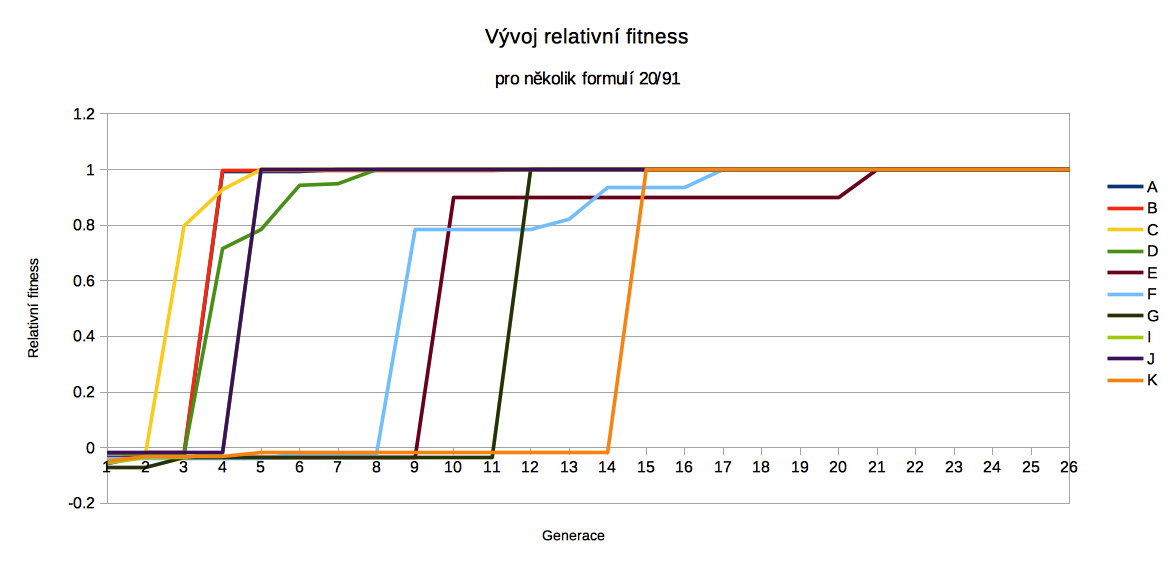
\includegraphics[scale=1]{graf-vyvoj-20-91.png} 
file:///Users/Tom/MI-PAA/task5/zprava_ukol5/graf-vyvoj-50-148.png
file:///Users/Tom/MI-PAA/task5/zprava_ukol5/graf-vyvoj-nesplnitelna.png

	-graf vývoje f na 20/91
	-graf vývoje f na 50/148
	-graf vývoje f prvního a druhého prvku na nesplnitelné formuli

	
\section{Závěr}
 %RESETOVAT SMC!!!!!!!!!!!
 %vybrat rýžovar
 %objednat Hue
 %skočit pro rježi


\end{document}